\chapter{Adaptive qMRI Sequence Design with Reinforcement Learning}
\label{ch:adaptive-rl}

%%%%%%%%%%%%%%%%%%%%%%%%%%%%%%%%%%%%%%%
% IMPORTANT
\begin{spacing}{1} %THESE FOUR
\minitoc % LINES MUST APPEAR IN
\end{spacing} % EVERY
\thesisspacing % CHAPTER
% COPY THEM IN ANY NEW CHAPTER
%%%%%%%%%%%%%%%%%%%%%%%%%%%%%%%%%%%%%%%

\setlength{\textfloatsep}{9pt plus 2pt minus 2pt}
\setlength{\floatsep}{7pt plus 2pt minus 2pt}
\setlength{\intextsep}{7pt plus 2pt minus 2pt}
\setlength{\abovecaptionskip}{3pt}
\setlength{\belowcaptionskip}{0pt}

\section{Chapter aim}
\label{sec:e2-chapter-aim}

The previous chapters established the simulator and digital phantom. This
chapter uses them for the central adaptive acquisition experiment: can a
reinforcement learning (RL) agent choose inversion-recovery spin-echo blocks
that estimate $T_1$ more efficiently than a fixed protocol?

This chapter addresses C2 and C3 from Chapter~\ref{ch1}. C2 is the compute
problem: a full KomaMRI Bloch simulation is too slow to use naively inside RL.
C3 is the adaptive design problem: the best next acquisition should depend on
what has already been measured, not only on a fixed protocol chosen before the
scan. The main technical contribution is therefore a multi-fidelity RL training
loop, plus a controlled evaluation of when adaptivity actually helps.

The conclusion is deliberately nuanced. On the full 14-sphere $T_1$ plate, the
agent learned a non-collapsed adaptive policy, but strong fixed schedules still
beat it. On a smaller five-sphere continuous-$T_1$ task, where the episode
really changes from scan to scan, the RL policy does beat the matched fixed
log-grid comparator. This is the positive adaptive result, but it should not be
overstated as a solution to the full 14-sphere mapping problem.

\section{Position relative to adaptive MRI work}
\label{sec:e2-related-position}

This chapter sits between three related literatures: adaptive model-based MRI,
automated sequence design, and reinforcement-learning control of MRI scanners.
It is not the first work to adapt an MR acquisition, nor the first work to use
machine learning for sequence design. The narrower contribution is a
simulation-in-the-loop RL environment for qMRI in which the agent controls a
spatially encoded 2-D acquisition of a calibrated phantom, receives fitted
tissue-parameter estimates during the scan, and is evaluated against fixed qMRI
protocols.

\begin{table}[!htbp]
\centering
\scriptsize
\setlength{\tabcolsep}{4pt}
\renewcommand{\arraystretch}{0.96}
\begin{tabularx}{\linewidth}{>{\raggedright\arraybackslash}p{2.7cm}
>{\raggedright\arraybackslash}p{4.2cm}
>{\raggedright\arraybackslash}X}
\toprule
Work & What it demonstrates & Critical comparison \\
\midrule
Adaptive model-based MR~\cite{adaptive_mri:23} &
Bayesian update of tissue-parameter uncertainty during a real-time multi-echo
experiment, with simulation, phantom and healthy-volunteer validation &
Stronger external validation than this project, including real hardware. It is
not an RL controller, and the reported task is a model-based adaptive T2/MRS
experiment rather than RL control over a 2-D qMRI phantom acquisition. \\
\addlinespace
MRzero~\cite{MRISeqSupLearning:21} &
End-to-end differentiable optimisation of sequence parameters, including a
clinical 3T scanner demonstration &
Much stronger hardware evidence. However, the optimisation is supervised and
offline: it learns a sequence, not a closed-loop policy that changes actions from
the current fitted tissue estimates. \\
\addlinespace
AUTOSEQ~\cite{zhu2018autoseq} &
Bayesian RL-style search over sequence actions in preliminary 1-D physics
simulation experiments &
Important early evidence that MR sequence design can be framed as sequential
control, but the task is deliberately simplified. It does not evaluate adaptive
qMRI estimation on a spatially encoded calibration phantom. \\
\addlinespace
Walker-Samuel~\cite{Walk_RL_CONTROL_MRI:19} &
DDPG control of a simulated scanner for task-specific active sensing and
shape classification &
The closest direct deep-RL comparator. It shows an RL agent can actively choose
scanner actions, but the objective is shape classification, not calibrated
parameter mapping. Walker-Samuel's task is more open-ended in one important
respect: the agent has to discover useful scanner behaviour from lower-level
controls. This project gives the agent higher-level IR-SE building blocks and a
fitter. The trade-off is realism of the quantitative evaluation: this chapter
uses 2-D k-space reconstruction, a digital QalibreMD phantom, noise, and fitted
$T_1$ error as the reward. It is still weaker because it remains simulator-only. \\
\addlinespace
MRF optimisation~\cite{Jordan_MRF_AUTO:21,mehta_mrf_review:2019} &
Offline design of time-varying schedules for multi-parameter fingerprints &
Directly relevant to quantitative imaging and multi-parameter contrast, but the
schedule is fixed before acquisition. The missing ingredient, which this chapter
tests in a narrower T1 setting, is observation-conditioned adaptation during the
scan. \\
\bottomrule
\end{tabularx}
\caption{Position of this chapter relative to the main adaptive and automated
MRI sequence-design papers discussed in Chapter~\ref{ch2}. The comparison is not
a claim that this work is broadly superior: existing adaptive MR and MRzero have
stronger hardware validation, while this chapter contributes a more realistic
deep-RL qMRI control setting than the closest prior RL scanner-control work.}
\label{tab:e2-related-position}
\end{table}

The key distinction is therefore methodological rather than absolute
performance. Compared with the strongest hardware-validated papers, this project
is less mature because every result is still simulated. Compared with the
closest RL scanner-control work, it is more structured but more quantitative:
the agent is not discovering arbitrary pulse-sequence behaviour from scratch,
because the sequence family and fitter are supplied. Instead, it must improve
fitted relaxation estimates after a 2-D k-space acquisition of known phantom
materials. The positive Run B result should be read in that context: it is
evidence that RL can learn a useful closed-loop qMRI timing strategy in a more
realistic evaluation pipeline, not proof that it is already ready for scanner
use.

\section{Environment formulation}
\label{sec:e2-env}

Each episode simulates a 2-D inversion-recovery spin-echo acquisition through
the T1 plate of the digital phantom. At each decision point the agent chooses
the timing of the next block. The reported runs use $N_\mathrm{pe}=32$,
$N_\mathrm{fe}=64$, 1 mm sphere voxels, full background water at target
fidelity, and fixed echo time $\mathrm{TE}=20$ ms. The scan-time budget is
240 s for the main experiments in this chapter. Since one phase-encode line is
acquired per shot, each block costs approximately
$N_\mathrm{pe}\cdot \mathrm{TR}$ seconds.

\paragraph{Noise model.} Independent complex Gaussian noise with absolute
standard deviation $\sigma=50$ is added to every k-space sample. The value is
calibrated, not arbitrary: the signal scale is a sum over simulated spins, so
the $\sigma\!\to\!\mathrm{SNR}$ map depends on voxel size, slice geometry and
matrix size, and must be derived at the training configuration. At this
geometry $\sigma=50$ gives a NEMA MS-1 dual-acquisition SNR of ${\approx}17$
averaged across the T1 plate at the reference block, rising to ${\approx}28$
on the brightest spheres (measured by \texttt{scripts/e2\_snr\_report.jl}).
This sits squarely in reported clinical inversion-recovery image quality: a
normal-brain FLAIR study measured mean tissue SNRs of 16--30 at 1.5T across
the structures analysed \cite{sohn2010flair}, while broader fMRI SNR work
 emphasises the dependence of SNR on voxel volume and acquisition design \cite{murphy2007howlongscan}.
The agent is therefore stressed with clinically realistic noise rather than an
arbitrary level. A 25-seed noise sweep
(Appendix~\ref{app:noise-calibration}) further shows that T1 fits degrade
gracefully up to $\sigma\approx85$ and collapse beyond, so $\sigma=50$ leaves
the task noise-limited but not estimation-broken.


\paragraph{Action space.} The policy outputs a vector in $[-1,1]^n$ which the
wrapper maps to physical timings. The bounds were fixed from the phantom and
pulse physics rather than tuned:
\begin{itemize}
\setlength{\itemsep}{1pt}
    \item $\mathrm{TI} \in [0.01, 3.0]$ s, chosen to bracket the plate's
    inversion nulls (where signal contrast and $T_1$ information peak), from
    the shortest sphere's ${\approx}17$ ms null ($T_1\ln 2$ at $T_1 = 24$ ms)
    to the longest's ${\approx}1.3$ s ($T_1 = 1.88$ s). By 3 s the longitudinal
    magnetisation has nearly fully recovered for every sphere, so the signal is
    insensitive to $T_1$. The 10 ms
    floor is not a hard physical limit (RF pulses occupy ${<}1$ ms at
    $B_1 = 20\,\mu$T) but is realistic and never binds.
    \item $\mathrm{TE} \in [5, 80]$ ms, fixed at 20 ms in all reported runs:
    TE carries $T_2$, not $T_1$, information, and freezing it removes a
    degree of freedom that only dilutes exploration on this task.
    \item $\mathrm{TR} \in [0.5, 5.0]$ s. The upper bound does not reach full
    recovery for the longest sphere (the $5\,T_1$ rule of thumb would want
    ${\approx}9.4$ s at $T_1 = 1.88$ s): the intended regime is steady-state
    partial recovery, never a fully relaxed start. The fitter models that
    partial recovery (the generalised IR model of
    Chapter~\ref{ch:mri-system-phantom}), so short-TR blocks are genuinely
    informative rather than merely corrupted, and the agent trades recovery
    against the $N_\mathrm{pe}\cdot\mathrm{TR}$ block cost.
    \item $\alpha \in [5^\circ, 90^\circ]$ when learned (Run A), spanning the
    full Ernst regime.
\end{itemize}
TI uses a logarithmic action mapping,
$\mathrm{TI}(u) = \mathrm{TI}_{\min}(\mathrm{TI}_{\max}/\mathrm{TI}_{\min})^{u}$
for $u\in[0,1]$, giving constant action resolution per decade of $T_1$; under
a linear map the informative TIs for the shortest spheres occupy roughly the
bottom $1.5\%$ of the interval, which starves them of policy resolution. In
the later five-sphere ablations $\alpha$ was fixed at $90^\circ$. This was an
evidence-based simplification: in Run A the learned flip angles collapsed to
$90^\circ$, and the Cramer--Rao fixed-schedule baseline independently chose
$90^\circ$ because it reduced the CRLB. The flip-angle degree of freedom was
therefore redundant for these T1 experiments, and later runs spent the
capacity on timing decisions rather than re-learning the same boundary
solution.

\paragraph{Action repair.} The environment repairs infeasible timing requests
rather than terminating the episode: the executed repetition time is
\[
    \mathrm{TR}_\mathrm{exec} = \max\!\left(\mathrm{TR}_\mathrm{req},\;
    0.5,\; (\mathrm{TI}+\mathrm{TE})/0.9\right),
\]
i.e.\ TR must contain the inversion and echo with 10\% headroom. Hard
rejection would be cleaner semantically, but early random policies would burn
rollouts learning the action-space geometry instead of sequence design, and
the resulting penalties push PPO towards conservative long-TR choices. The
guardrail is audited rather than hidden: every step emits both requested and
executed timings plus a repaired flag, and the evaluation scripts report
repair rates and mean TR lift. A policy that leans on the repair is therefore
detectable; the reported Run B 240 s policy executes zero repairs, and the
560 s policies repair 0.3--1.8\% of blocks.

\paragraph{Observation.} The observation is deliberately compact:
$\log_{10}$ of the running per-sphere $T_1$ estimates (a zero sentinel before
the first valid fit, which requires at least two measurements), the fraction
of scan time used, the fraction of blocks used, and a constant bias input.
Observations and rewards are normalised online with clipping at $\pm10$. The
agent never sees the reconstructed image or raw k-space: it acts only on the
fitter's $T_1$ estimates and budget, the same interface a qMRI pipeline would
expose. This keeps the policy on the genuine estimation objective rather than
on simulator-specific pixel patterns that may not generalise to real hardware.
Some ablations append an uncertainty proxy from the fitter
(Section~\ref{sec:e2-ablations}); the main 240 s result does not. After each
block, the environment reconstructs the image, extracts each sphere's
region-of-interest signal, refits $T_1$, and computes the reward. The main
reward is the improvement in log-MAPE:

\[
    r_t =
    \log\!\left(\mathrm{MAPE}_{t-1} + \epsilon\right)
    - \log\!\left(\mathrm{MAPE}_{t} + \epsilon\right).
\]

This reward is dense and local: it rewards a block for reducing the current
estimation error, rather than only awarding a terminal score. This was important
because an initial single-voxel experiment (not reported here) collapsed to a
nearly fixed policy when a large terminal bonus made it sufficient to finish the
episode rather than optimise the measurement sequence.

Training uses PPO~\cite{schulman_ppo_2017}. PPO was chosen because it is a
robust on-policy baseline and can be used with continuous actions without
needing a replay buffer. This matters for the Python--Julia simulator loop:
each rollout step triggers simulator, reconstruction, fitting, and reward code
across the Python--Julia boundary. During development, a simple on-policy
learner made it easier to diagnose whether failures came from the MRI model,
the fitter, the reward, or the policy update itself.

\section{Multi-fidelity curriculum}
\label{sec:e2-mf-method}

\subsection{The cost wall and the fidelity ladder}
\label{sec:e2-mf-ladder}


The main engineering difficulty is simulator cost. Every environment step
triggers a multi-shot Bloch simulation of the whole phantom, followed by 2-D
reconstruction and a refit. The cost is set mainly by how many RF pulses the
integrator must resolve: KomaMRI steps through the free-precession delays
(TI, TR) with large time steps, but each RF pulse needs fine time
discretisation, so the per-step cost scales with the number of shots
$N_\mathrm{pe}$ (one excitation and refocusing pulse per phase-encode line) and
the spin count $n_\mathrm{spins}$, and only weakly with the requested timing.
At the target configuration (T15, $64\times32$, 1 mm voxels, 1 mm slab through
the T1 plate) the sliced phantom contains 23{,}735 spins, of which 18{,}919
(80\%) are background water. The sphere material that the agent actually
measures is only 4{,}816 spins. A full-Bloch step measured about 4 s on CPU, so
a 200k-step PPO run is roughly nine days of simulation before any evaluation
overhead. The reported Run B family was trained on GPU, where the same stages
ran some $5$--$7\times$ faster (${\approx}0.06$ s/step at the cached and
coarse-water stages); extrapolated by spin count to the 1 mm full plate this is
still ${\approx}0.2$ s/step, leaving a single-fidelity full-Bloch run on the
order of a day before evaluation overhead. Single-fidelity full-Bloch training
therefore does not fit the project compute budget on either device.

Because 80\% of the spins are water, both cost levers target the water:
\emph{coarsen} it or \emph{cache} it. Coarsening reuses the digital twin's
independent water grid (Chapter~\ref{ch:mri-system-phantom}): water spins are
laid out on a coarser grid with proton density rescaled to conserve total
magnetisation, and a 3 mm water grid cuts the water spin count by $9\times$
(18{,}919 $\to$ 2{,}103), taking the phantom to 6{,}919 spins. Caching,
described next, removes the water from the per-step simulation entirely.
Together with the analytic surrogate these give the ladder in
Table~\ref{tab:e2-fidelity-ladder}, spanning a ${\sim}30\times$ per-step cost
range.

\begin{table}[!htbp]
\centering
\small
\setlength{\tabcolsep}{4pt}
\renewcommand{\arraystretch}{0.92}
\begin{tabular}{llrrl}
\toprule
Fidelity & Water model & Bloch spins & s/step & Main bias \\
\midrule
\texttt{analytic} & closed form & 0 & 0.034 & no reconstruction, no water crosstalk \\
\texttt{cached3} & cached template, 3 mm & 4{,}816 & 0.34 & cached and coarse water \\
\texttt{cached} & cached template, 1 mm & 4{,}816 & ${\approx}$0.34 & cached water, target geometry \\
\texttt{full3} & full Bloch, 3 mm & 6{,}919 & 0.42 & coarse water discretisation \\
\texttt{full} & full Bloch, 1 mm & 23{,}735 & 1.03 & target fidelity \\
\bottomrule
\end{tabular}
\caption{Fidelity ladder used for E2. ``Bloch spins'' is the number simulated
per step at the 14-sphere plate (exact counts from
\texttt{scripts/e2\_spin\_counts.jl}; the cached rungs Bloch-simulate only the
4{,}816 sphere spins and add the water from the template); s/step are measured
Run A CPU stage averages, set mainly by $N_\mathrm{pe}$ and the spin count
rather than the requested timing. The \texttt{cached} rung costs
the same as \texttt{cached3} because the template add is resolution-independent;
its standalone benchmark measured $8.0\times$ versus matched full Bloch. Lower
rungs are cheaper but biased; Section~\ref{sec:e2-mf-switch} ensures the bias
cannot validate itself.}
\label{tab:e2-fidelity-ladder}
\end{table}

\subsection{Cached water: exploiting simulator linearity}
\label{sec:e2-water-cache}

The cached rungs rest on two exact structural facts. First, the Bloch
simulation is linear in spins, so the acquired k-space separates exactly:
\[
    S_\mathrm{full} = S_\mathrm{spheres} + S_\mathrm{water}.
\]
Second, the water is a single homogeneous material, so its contribution to
phase-encode line $k$ (acquired on shot $k$) factorises into a scalar shot
amplitude and a fixed geometric profile:
\[
    S_\mathrm{water}[k,:] = M_z^{(k)}(\mathrm{TI},\mathrm{TR},\alpha)\,
    \sin\alpha \,\; W_\alpha[k,:].
\]
Here $M_z^{(k)}$ is the water's longitudinal magnetisation at the $k$-th
excitation, available in closed form from the same transient recovery model
the fitter inverts, and $W_\alpha$ is a template capturing everything
geometric --- spin positions and Fourier encoding, $T_2$ decay at the
reference echo time, static $B_0$ phase. The template is obtained once, by
running a single Bloch simulation of the water alone and dividing the
$M_z^{(k)}\sin\alpha$ factor out of each k-line.

Evaluating a new $(\mathrm{TI},\mathrm{TR})$ then costs $O(N_\mathrm{pe})$
arithmetic for the new $M_z^{(k)}$ plus a row-wise rescale of the template;
only the sphere spins are re-simulated. This is the ${\sim}8\times$ per-step
saving of the cached rungs. The alternative of modelling the water
analytically as well is measurably too crude: it leaves visible
reconstruction and crosstalk residuals and per-sphere $T_1$ deviations from
the full simulation of up to ${\sim}40\%$, whereas the cached model matches
full-Bloch $T_1$ fits to $0.12\%$ on average (worst sphere $1.15\%$, the
fitter's discrete-grid floor). Appendix~\ref{app:water-cache} shows the
validation images and fits.

The flip angle is the subtle part: the factorisation is exact only at the
$\alpha$ the template was built with. Two effects were measured. First, the
closed-form transient mis-scales across $\alpha$: at $90^\circ$,
$\cos\alpha=0$ and every shot starts from the same thermal state, but at
$30^\circ$ residual magnetisation carries between shots and the ratio of
simulated to analytic per-shot amplitude drifts from 1.01 on the first
k-line to 1.40 on the sixteenth. Second, the template itself changes with
$\alpha$ through spoiling and echo formation, by 7--21\% spatially between a
$30^\circ$ and a $90^\circ$ template; this error is TI-independent, so no TI
rescaling can correct it. The implementation therefore stores a \emph{bank}
of $\alpha$-matched templates on a grid spanning the action range. At a
matched $\alpha$ a template is exact to ${\sim}10^{-8}$ relative k-space
error; an off-grid $\alpha$ is evaluated by computing the two bracketing
templates, each at its own $\alpha$, and blending linearly in $\alpha$. A
template is never rescaled to a different flip angle analytically --- that
would reintroduce exactly the error the bank exists to avoid.

One constraint follows from the construction: the template is keyed to the
spin positions, so the cached rungs hold the phantom pose fixed, while the
full-Bloch rungs and all full-fidelity probes apply the in-plane pose jitter.
Cheap stages therefore optimise under slightly narrower conditions than the
target measures --- a stated fidelity compromise, accepted because every
promotion and checkpoint decision is scored on the full environment.

\subsection{The switch rule: bias-aware promotion}
\label{sec:e2-mf-switch}

Warm-starting between fidelities is mechanically trivial; the design question
is \emph{when} to promote. Fixed per-stage step counts are impossible to
justify and waste budget. The switch rule adapts two ideas from
multi-fidelity RL: Sifaou and Simeone select the fidelity with the best
expected information gain about the target policy per unit simulation
cost~\cite{sifaou_mf_hrl_2025}, and Cutler, Walsh and How promote when
lower-fidelity samples stop being useful for the real
task~\cite{cutler_multifidelity_2015}. Neither is implemented literally as
this project maintains no posterior over policies, but their shared
principle fixes the central design decision: \textbf{promotion is driven by
held-out full-simulator validation, never by the cheap simulator's own
score.} A biased simulator can keep improving its own score by exploiting its
bias, the same failure mode as the single-voxel fitter exploit, so a cheap rung may
generate rollouts but may not certify its own policy.

Concretely, every fourth PPO rollout (2{,}048 steps at
$n_\mathrm{steps}=512$) the current policy is probed for four episodes on the
current-fidelity environment and four on the full environment, with identical
seeds. The full-probe score is
\[
    P_H = -\log_{10}\!\left(\mathrm{clamp}(\mathrm{MAPE}_H,
    10^{-3}, 1)\right),
\]
where the clamp models each rung's accuracy floor so a saturated cheap stage
reads as flat. After a per-stage minimum-step gate, the trainer promotes out
of a cheap stage when any of four signals fires:
\begin{enumerate}
\setlength{\itemsep}{1pt}
    \item \textbf{Target plateau} (primary): the relative gain in $P_H$ over
    the last three decision points falls below 2\% --- the cheap rung has
    given what it can.
    \item \textbf{Ranking breakdown}: the Spearman correlation between
    cheap-probe and full-probe MAPE across the stage's decision points falls
    below a per-rung guardrail (0.7 for \texttt{analytic}, 0.8 for the cached
    rungs, 0.9 for \texttt{full3}), evaluated only once at least four points
    exist. A cheap rung may be biased, but it must still \emph{rank} policies
    like the target.
    \item \textbf{Bias intolerance}: the cheap/full probe gap exceeds one
    percentage point of mean MAPE or two points of p90.
    \item \textbf{Budget reserve}: remaining wall-clock falls to the 20\% of
    the total budget reserved for the final full stage. This overrides every
    other gate, guaranteeing the target fidelity always receives compute.
\end{enumerate}
Each stage also has a hard step cap, and the whole curriculum runs under a
hard wall-clock deadline (9 h for the reported runs). On every promotion the
\emph{fidelity gap} is recorded --- the full-probe MAPE of the warm-started
policy before any training at the new rung, minus the previous stage's final
value --- as a direct transfer diagnostic. The decision logic is a pure
Python module, unit-tested on synthetic metric histories separately from the
PPO and Julia orchestration, and every decision is appended to a JSON history
together with the signal that fired, so each run's switching behaviour can be
audited afterwards.

% in practice the bias intolerance was probably set too tight.
\subsection{Next-fidelity lookahead (V2)}
\label{sec:e2-mf-lookahead}

The plateau rule has a blind spot: it says the current rung is exhausted, not
that the next rung will help. The V2 controller adds a cheap empirical test
before promoting on progress grounds. A lookahead is triggered when the
recent slope of $P_H$ per wall-clock second falls below $0.25\times$ the
stage's previous best slope (a scale-free collapse test that transfers across
hardware), or when the relative gain comes within $2\times$ of the plateau
threshold. The trainer then \emph{clones} the policy into a fresh PPO
instance attached to the next-fidelity environment --- weights copied,
observation-normalisation statistics deep-copied, reward normalisation reset
--- trains the clone for a single rollout (512 steps, ${\sim}230$ s at
\texttt{full3} in Run A), and re-scores it on the same full-probe seeds.
Promotion on slope grounds happens only if the clone's improvement per second
beats the current rung's by a factor of 1.15.

The lookahead carries its own guardrails: its cumulative wall-clock is capped
at 10\% of the total budget; it never runs into the final-stage reserve; and
the clone is discarded afterwards, never mutating the live model or its
normalisation statistics --- the real model reaches the next rung by warm
start, so the one-rollout clone is a probe, not a head start. The plateau
rule remains as the fallback, and the logged switch reason distinguishes a
lookahead-driven promotion from a fallback one.

\subsection{Stage hand-off and global-best checkpointing}
\label{sec:e2-mf-handoff}

Only the forward-model and water settings change between rungs; the
observation and action layout, reward, noise and resolution are held fixed so
the warm-started weights remain valid. The observation-normalisation
statistics carry across each switch --- the observation is physical
($\log_{10} T_1$ in seconds), so its running statistics are comparable across
fidelities --- but the reward normalisation is reset, because the reward
scale shifts with each rung's bias. Optionally the optimizer is also rebuilt
at each switch, so stale Adam moments from the previous rung do not distort
the first updates at the new one.

Finally, the trainer maintains a global-best checkpoint across the whole
curriculum, selected on the target fidelity. This was added after Run A
showed that the final policy of a curriculum can be worse than one it had
already passed through (Section~\ref{sec:e2-run-a}). Selection is two-tier
because four-episode probes are far too noisy to pick checkpoints: every full
probe (switch decisions, stage starts and ends, periodic stage evaluations)
only \emph{screens} candidates, and a candidate that beats the incumbent on
its screen is re-evaluated on twelve independent episodes at a separate seed
offset. Only a confirmed improvement overwrites the checkpoint, and its
metadata records both the screening and the confirmed scores. Report-grade
numbers are taken from neither: all tables in this chapter come from fresh
24-episode evaluations with confidence intervals.

\section{Run A: full 14-sphere T1 plate}
\label{sec:e2-run-a}

Run A was the first end-to-end V2 curriculum. It used the full 14-sphere T1
plate, a 240 s scan budget, $T15$ field values, $\sigma=50$, fixed TE, and
learned $\alpha$. The ladder was
\[
\texttt{analytic} \rightarrow \texttt{cached3} \rightarrow
\texttt{full3} \rightarrow \texttt{full}.
\]
The run was trained under a 9 h wall-clock budget.

\begin{table}[!htbp]
\centering
\small
\setlength{\tabcolsep}{4pt}
\renewcommand{\arraystretch}{0.92}
\begin{tabular}{lrrrr}
\toprule
Stage & Steps & Wall [h] & s/step & End full-Bloch MAPE \\
\midrule
\texttt{analytic} & 8.2k & 0.08 & 0.034 & 16.60\% \\
\texttt{cached3}  & 41.0k & 3.28 & 0.338 & \textbf{10.37\%} \\
\texttt{full3}    & 73.7k & 3.94 & 0.416 & 14.03\% \\
\texttt{full}     & 79.5k & 1.64 & 1.03  & 12.26\% \\
\bottomrule
\end{tabular}
\caption{Run A stage summary. The productive stage was \texttt{cached3}; moving
to \texttt{full3} degraded the target-fidelity score, and the final full stage
did not recover the best cached checkpoint.}
\label{tab:run-a-stages}
\end{table}

\begin{figure}[!htbp]
\centering
\begin{minipage}[c]{0.50\linewidth}
\centering
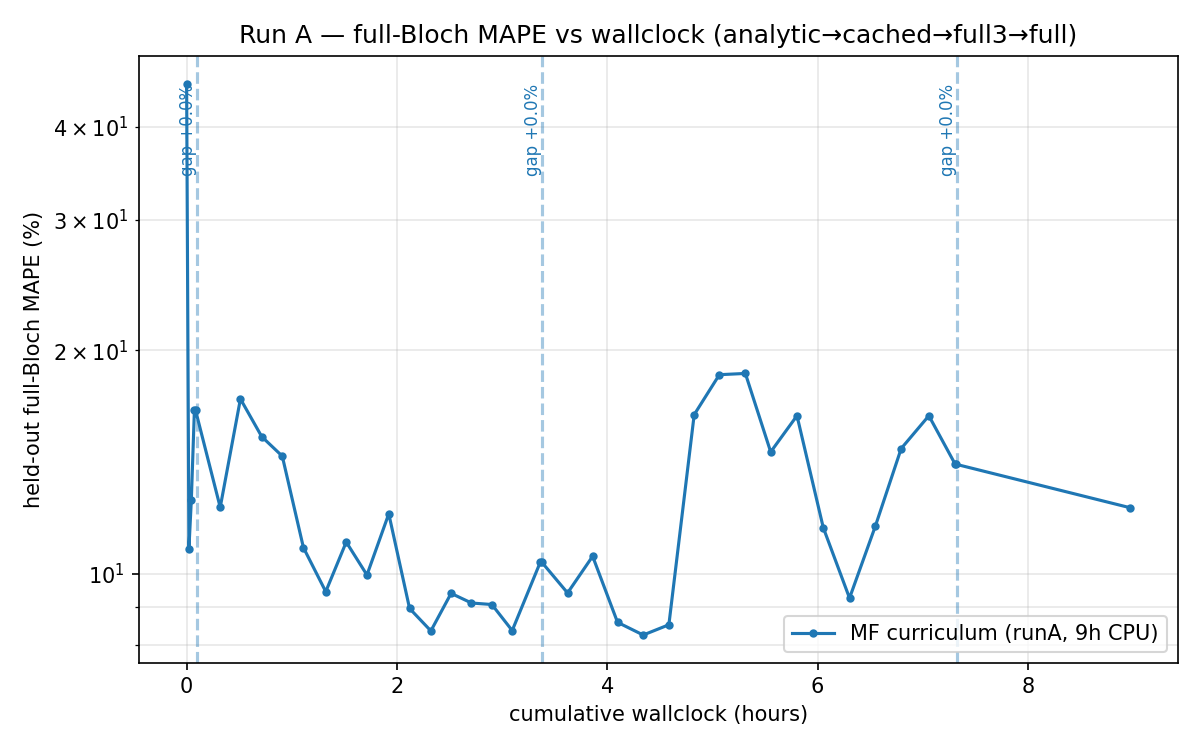
\includegraphics[width=\linewidth]{imgs/e2_rl/runA_moneyplot.png}
\end{minipage}\hfill
\begin{minipage}[c]{0.46\linewidth}
\centering
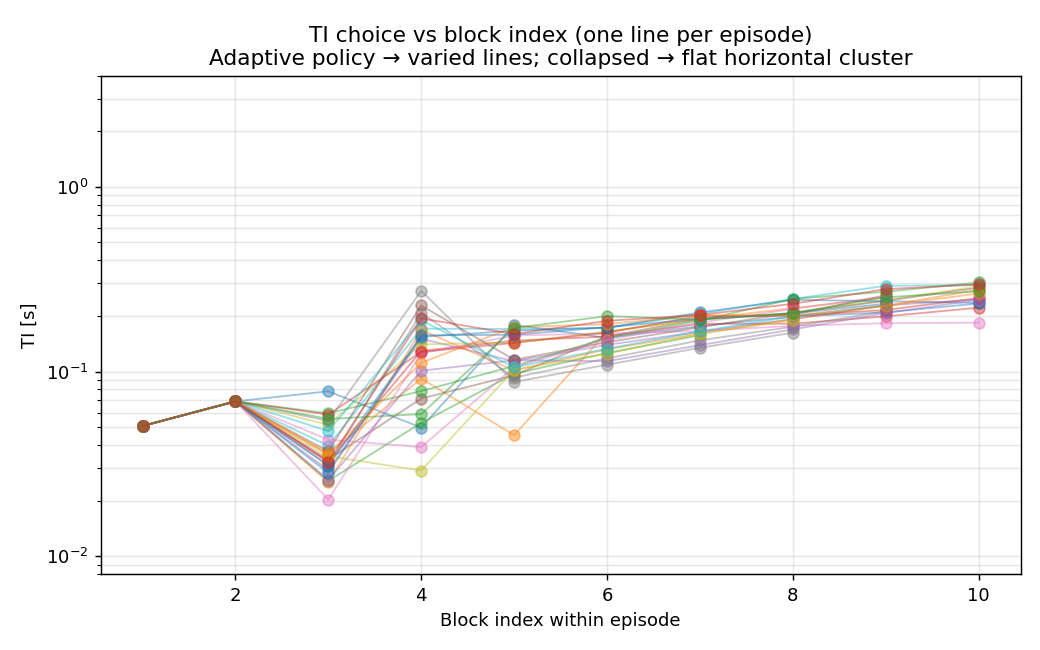
\includegraphics[width=\linewidth]{imgs/e2_rl/runA_ti_per_episode.png}
\end{minipage}
\caption{Run A curriculum behaviour. Left: full-Bloch probe MAPE versus
wall-clock time. The cached-water stage reached the best basin, then full3
regressed. Right: the learned policy was not collapsed; TI varies across
episodes and within an episode, but the final policy still under-sampled the
long-T1 regime.}
\label{fig:run-a-behaviour}
\end{figure}

Figure~\ref{fig:run-a-behaviour} is the main diagnostic, and the logged switch
reasons make the controller's behaviour concrete. The analytic stage was left
on a \emph{ranking breakdown} (the cheap probe stopped ordering policies like
the full probe) after 8.2k steps; it had already collapsed the full-probe MAPE
from ${\approx}42\%$ to ${\approx}10\%$ essentially for free. The
\texttt{cached3} stage was left on a \emph{target plateau} at 41k steps, having
improved the full-probe score into an 8--10\% basin --- the best the run ever
reached. The problem occurred after the switch to \texttt{full3}: the
target-fidelity score jumped back up and ended worse than the cached basin, and
that stage was only left on the \emph{budget reserve} override at 74k steps,
handing the last 20\% of wall-clock to the \texttt{full} stage. The 3 mm-water
full-Bloch environment was therefore not a harmless bridge to the 1 mm target;
its optimum differs from the 1 mm optimum the probe scores (rank correlation
${\approx}0.6$, bias ${\pm}5\%$).

The lookahead mechanism gave a useful warning at exactly this boundary. When
the \texttt{cached3} slope collapsed, the controller cloned the policy, trained
it for one rollout (${\approx}230$ s) at \texttt{full3}, and re-scored it: the
clone's full-Bloch MAPE got \emph{worse} (10.37\% $\to$ 11.69\%), so the slope
gain was ${\approx}0$ and the rule correctly \emph{declined} to promote on
slope grounds. The plateau fallback promoted anyway, and the regression the
lookahead had predicted in 230 s then played out over the whole 3.9 h stage.
This is an informative negative result: the V2 signal was meaningful, but the
controller's action space did not include ``skip this rung and keep the global
best'', which is what the evidence called for.

Run A was evaluated on a strict seed-600000 held-out set. This seed was not used
for policy training, curriculum switching, or checkpoint selection, so the
negative result in Table~\ref{tab:run-a-current-comparison} is not a validation
leakage artefact.

\begin{table}[!htbp]
\centering
\scriptsize
\setlength{\tabcolsep}{3pt}
\renewcommand{\arraystretch}{0.92}
\begin{tabular}{lrrrr}
\toprule
Policy or schedule & Mean MAPE & 95\% CI & p90 & Mean time \\
\midrule
\texttt{cr\_optimal\_alpha} fixed schedule & \textbf{4.70\%} & [4.42, 5.00] & \textbf{5.68\%} & 240 s \\
\texttt{log\_grid\_trmatched} fixed schedule & 5.80\% & [5.24, 6.40] & 8.06\% & 218 s \\
Run A cached-best checkpoint & 9.44\% & [8.18, 10.94] & 14.11\% & 231 s \\
Run A final policy & 11.68\% & [10.42, 13.03] & 15.22\% & 232 s \\
Run A analytic checkpoint & 16.03\% & [13.97, 18.56] & 20.87\% & 223 s \\
\bottomrule
\end{tabular}
\caption{Run A comparison on 24 strict seed-600000 held-out evaluation episodes.
The agent was adaptive, but the fixed schedules were better on the full
14-sphere task.}
\label{tab:run-a-current-comparison}
\end{table}

The learned policy was nevertheless not the degenerate fixed-policy failure
mode. Diagnostics over
24 episodes gave TI intra-episode log standard deviation 0.281, inter-episode
log standard deviation 0.290, and modal-bin share 11.9\%. The chosen TI also
correlated positively with the running estimate and with the most uncertain
sphere ($r=+0.50$ and $r=+0.64$ respectively). In other words, the policy was
using the state, not replaying one fixed list of actions.

The failure was more specific, and Table~\ref{tab:run-a-current-comparison}
reads as an unintended ablation of the curriculum itself: \emph{the cheap
stages delivered the result and the expensive stages eroded it.} The
\texttt{analytic} checkpoint scores 16.03\%, the \texttt{cached3}-best
checkpoint 9.44\% --- the best the run produced --- and the final policy only
11.68\%. The mechanism is visible in the learned TIs. The cached-best policy
had pushed its TI ramp up to ${\approx}0.8$ s, long enough to characterise the
mid-to-long-$T_1$ spheres, cutting Pool 2/3/4 ($T_1 = 1.43/1.03/0.75$ s) error
to 18.7/13.8/10.7\%. The two expensive stages then shrank the ramp back to
0.3--0.6 s and reduced intra-episode exploration (TI log-$\sigma$ 0.38 $\to$
0.28), re-inflating those same pools to 28.2/23.8/19.0\%. The longest sphere,
Pool 1 ($T_1=1.88$ s), was beyond reach for every checkpoint (${\approx}41\%$):
even the cached-best 0.8 s TIs fall short of its ${\approx}1.3$ s inversion
null, so this is an action-coverage ceiling, not only a training-time problem.

The flip-angle degree of freedom told a consistent story. It collapsed to the
$90^\circ$ bound and, if anything, the curriculum drove it there harder over
training ($\alpha$ std $2.4^\circ \to 1.6^\circ \to 0.0^\circ$ across the
checkpoints); the best fixed Cramer--Rao baseline also selected $90^\circ$.
This is why $\alpha$ was fixed in the later Run B family: both the learned
policy and the CRLB baseline indicated that the useful optimisation pressure
was in TI/TR timing, not flip-angle selection.

One caveat on the absolute numbers. The sibling digital twin was improved
mid-project (a random-phantom sampler and an SO3 pose sampler), so the same
saved Run A policy scores 11.68\% on the current simulator versus 10.16\% when
first analysed. Table~\ref{tab:run-a-current-comparison} re-evaluates every
policy and baseline on the \emph{current} simulator, so the comparison is
internally consistent; the cross-version shift is reported only to explain why
older logs differ.

The Run A interpretation is therefore:
\begin{itemize}
\setlength{\itemsep}{1pt}
    \item multi-fidelity training made the experiment computationally feasible;
    \item the policy learned a genuine state-dependent timing strategy;
    \item the final 14-sphere agent did not beat fixed schedules;
    \item global-best checkpointing is required because later fidelity stages can erase a useful cheap-stage policy;
    \item the full 14-sphere task rewards robust global coverage, so it is not the best test of closed-loop adaptivity.
\end{itemize}

\section{Run B: five-sphere continuous-T1 task}
\label{sec:e2-run-b}

Run B changes the task so that adaptivity has a fairer chance to matter. The
physical sphere labels are fixed at \(\{1,3,6,8,14\}\), covering the long, mid
and short ends of the T1 plate. However, their $T_1$ values are sampled
continuously each episode over the T15 phantom range, with $T_2$ and $T_2^*$
preserving their nominal ratios to $T_1$. The geometry is therefore stable, but
the realised relaxation distribution changes from scan to scan.

This is easier than the full 14-sphere problem, and it is important to say so.
It is not a replacement headline for full phantom mapping. Its purpose is to
test the specific adaptive claim: when the episode's tissue parameters vary,
can the agent use early measurements to choose a better later timing schedule
than a fixed grid?

The main completed Run B result is the 240 s no-uncertainty GPU run.
% Source run directory: runs/e2/mf_runB_cached3_cached_full3_full_gpu.
It used the ladder
\[
\texttt{analytic} \rightarrow \texttt{cached3} \rightarrow
\texttt{cached} \rightarrow \texttt{full3} \rightarrow \texttt{full}.
\]
The extra \texttt{cached} stage is the target-resolution cached-water bridge
missing from Run A. The reporting checkpoint is the global-best policy, not the
last policy.

\begin{figure}[!htbp]
\centering
\begin{minipage}[c]{0.49\linewidth}
\centering
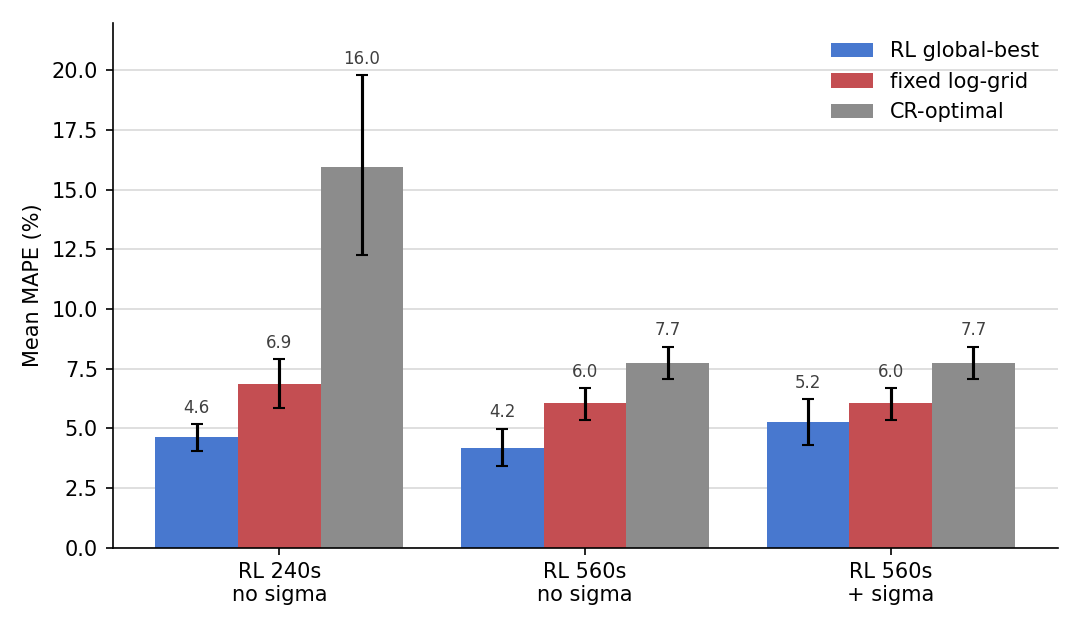
\includegraphics[width=\linewidth]{imgs/e2_rl/runB_mape_comparison.png}
\end{minipage}\hfill
\begin{minipage}[c]{0.49\linewidth}
\centering
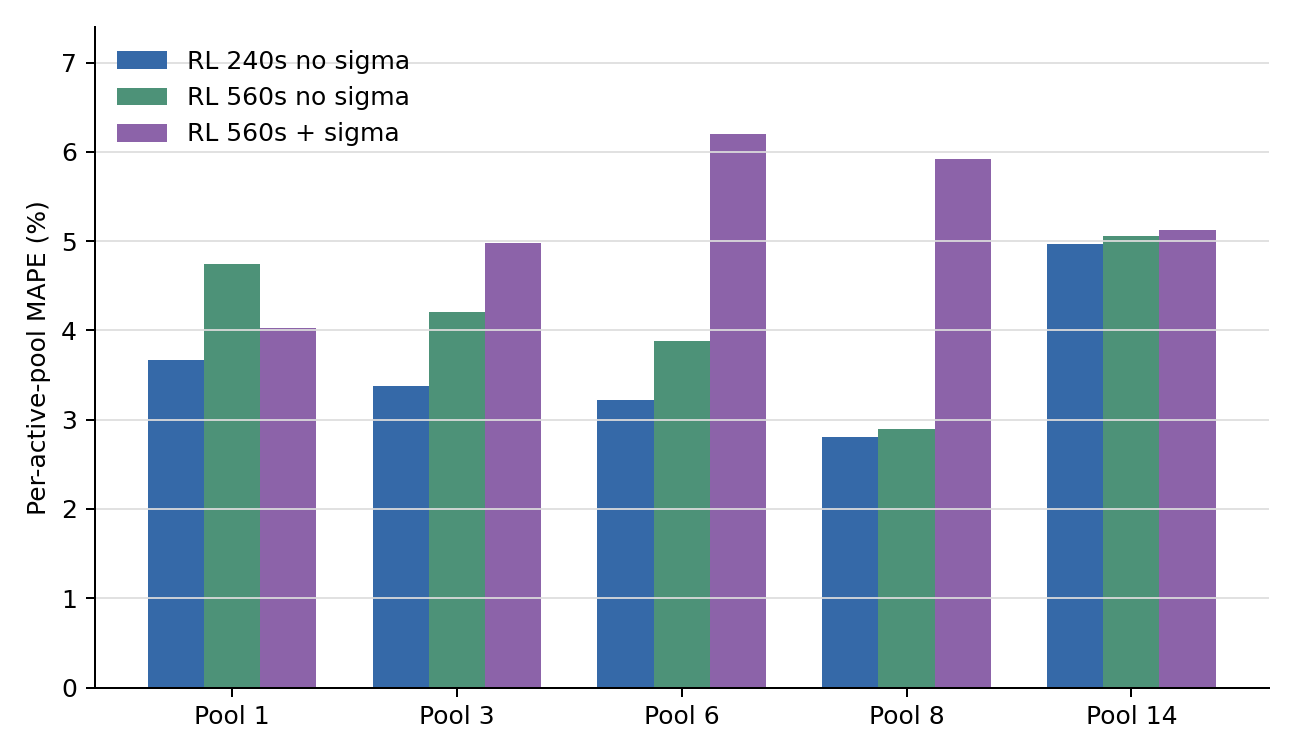
\includegraphics[width=\linewidth]{imgs/e2_rl/runB_per_pool.png}
\end{minipage}
\caption{Run B five-sphere results. Left: global-best RL policies compared with
the matched fixed log-grid baseline. The 240 s result is baseline-comparable but
not a strict held-out seed; the 560 s bars use strict held-out evaluation. Right:
per-active-pool MAPE for the RL policies.}
\label{fig:run-b-results}
\end{figure}

\begin{table}[!htbp]
\centering
\small
\setlength{\tabcolsep}{3pt}
\renewcommand{\arraystretch}{0.92}
\begin{tabular}{lrrrr}
\toprule
Policy or schedule & Mean MAPE & 95\% CI & p90 & Success $<5\%$ \\
\midrule
Run B RL global best & \textbf{3.61\%} & [3.26, 3.98] & \textbf{4.55\%} & \textbf{91.7\%} \\
Run B RL final policy & 4.19\% & [3.82, 4.58] & 5.26\% & 83.3\% \\
Fixed \texttt{log\_grid\_trmatched} & 5.60\% & [5.09, 6.13] & 7.08\% & -- \\
\bottomrule
\end{tabular}
\caption{Run B 240 s five-sphere result on 24 seed-500000 evaluation episodes.
This seed was also used by training evaluation, so the result should be
confirmed with a strict held-out seed before becoming the sole headline table.
It is nevertheless the matched comparison against the available 240 s fixed
baseline.}
\label{tab:run-b-240}
\end{table}

The 240 s policy beats the matched fixed log-grid comparator by about two
percentage points of mean MAPE. The per-pool breakdown is also balanced: Pools
1, 3, 6, 8 and 14 scored 3.67\%, 3.38\%, 3.22\%, 2.81\% and 4.97\% MAPE
respectively. This matters because the result is not an average dominated by one
easy pool. The shortest-$T_1$ active pool remains the hardest, but it is still
below 5\% MAPE.

\begin{figure}[!htbp]
\centering
\begin{minipage}[c]{0.49\linewidth}
\centering
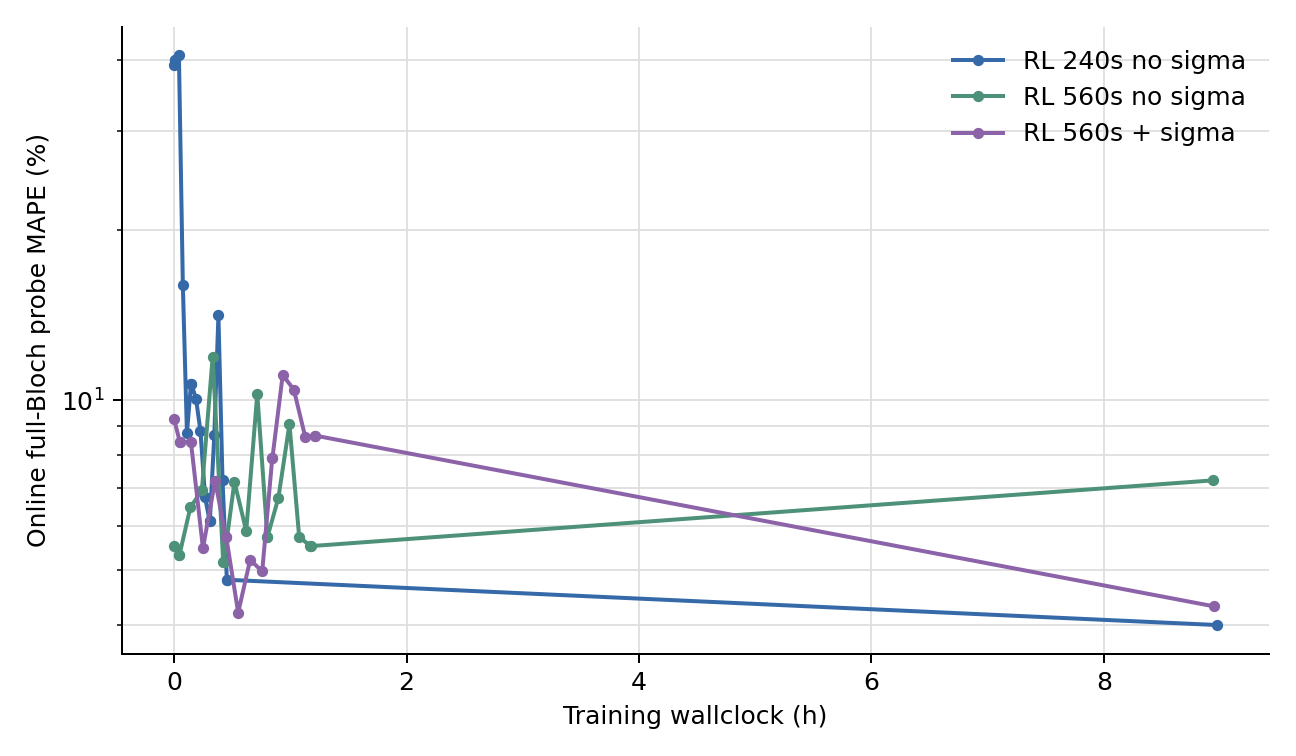
\includegraphics[width=\linewidth]{imgs/e2_rl/runB_curriculum_probes.png}
\end{minipage}\hfill
\begin{minipage}[c]{0.49\linewidth}
\centering
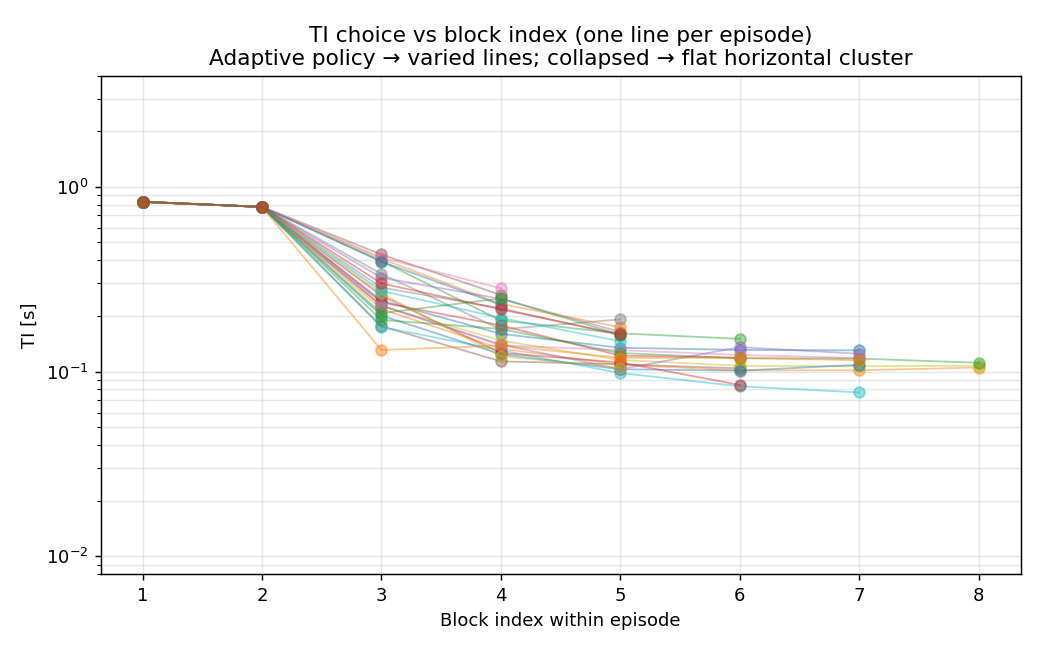
\includegraphics[width=\linewidth]{imgs/e2_rl/runB_240_ti_per_episode.png}
\end{minipage}
\caption{Run B 240 s policy behaviour. Left: full-Bloch probes during the
curriculum. The final full stage is noisy and global-best selection is needed.
Right: the global-best policy opens with a high-TI probe and then uses shorter
adaptive refinements.}
\label{fig:run-b-policy}
\end{figure}

The learned schedule in Figure~\ref{fig:run-b-policy} is qualitatively
different from Run A. The global-best 240 s policy uses 5.92 blocks on average,
with no timing repairs. It usually starts with two high-TI probes around
0.78--0.83 s and then moves to shorter refinements. The correlation between TI
and current $T_1$ estimate is negative ($r=-0.720$ for the main diagnostic),
which initially looks counter-intuitive. It is better interpreted as a
two-phase strategy: first buy a long inversion probe that is informative across
the sampled range, then shorten TI after the estimate has stabilised. This is a
real adaptive pattern, but it is not the simple monotonic rule ``higher current
$T_1$ implies longer next TI''.

The 240 s comparison shares its evaluation seed with the training stream, so
the cleanest statistical claim comes from a longer-budget control trained with
$\alpha$ fixed at $90^\circ$ and evaluated on a strict, never-seen
seed-600000 held-out set. At a 560 s budget the global-best RL policy scores
\textbf{4.16\%} MAPE ([3.41, 4.99], p90 6.64\%) against \textbf{5.86\%}
([5.24, 6.45], p90 8.02\%) for the matched fixed log grid on the same held-out
call --- the same ${\approx}1.7$ percentage-point advantage as at 240 s, now
without any train/eval seed overlap. The fixed log grid is essentially flat
from 240 to 560 s (5.60\% $\to$ 5.71\%), so the RL gain is not simply ``more
blocks'': the 560 s policy uses its ${\approx}14$ blocks (versus the fixed
grid's 10) in a different, closed-loop allocation, and the 240 s policy is the
stronger efficiency story, beating the fixed schedule with only ${\approx}6$
blocks and ${\approx}230$ s.

This is the strongest evidence for A3. The task was deliberately constructed so
that a fixed global schedule is less naturally optimal than in the 14-sphere
case, and the RL policy then found a compact closed-loop strategy that improved
both mean and p90 error against the fixed comparator at two budgets. The result
is still bounded: it rests on one training seed per arm, and the headline 240 s
global-best policy still needs a strict seed-600000 re-evaluation to fully
remove overlap with the training evaluation stream.

\section{560 s and ablation status}
\label{sec:e2-ablations}

The longer-budget and observation ablations are not yet mature enough for a
full results section, so they are summarised here.

\begin{itemize}
\setlength{\itemsep}{2pt}
    \item \textbf{560 s no-uncertainty control.} The global-best policy scored
    4.16\% MAPE on a strict 24-episode held-out evaluation, versus 5.86\% for
    the fixed log-grid comparator on the same held-out call. This supports the
    five-sphere adaptive result, but it is not a clean scan-time ablation of the
    240 s run because the 560 s runs fixed $\alpha=90^\circ$ while the 240 s run
    still learned $\alpha$.

    \item \textbf{560 s uncertainty-channel treatment.} Adding
    \(\log_{10}(\sigma_{T_1}/T_{1,\mathrm{est}})\) to the observation did not
    improve strict held-out performance. The global-best policy scored 5.25\%
    MAPE with p90 9.34\%, worse than the no-uncertainty control. The uncertainty
    proxy is therefore not a positive result. It may be too noisy early in the
    episode, when the fitter has only a few measurements.

    \item \textbf{Global best versus final policy.} The 560 s no-uncertainty run
    had an earlier confirmed global best near 3.45\% on the 12-episode
    confirmation eval, but the final policy drifted to 7.12\% on the
    seed-500000 24-episode eval. This reinforces the Run A lesson: the last
    policy is not automatically the best policy in a multi-fidelity curriculum.

    \item \textbf{Memory ablations.} Two memory mechanisms are planned but not
    yet report-grade: an executed-TI histogram in the observation and a recurrent
    PPO policy with an LSTM state. These test whether the current state
    \([T_{1,\mathrm{est}},\mathrm{budget}]\) is an adequate summary of the
    acquisition history. The hypothesis is concrete: two different TI histories
    can produce similar current fits, but have different information value for
    the next block.

    \item \textbf{ROI and reconstruction ablations.} ROI radius 1 was used for
    Run B to reduce centre-pixel sensitivity. A paired ROI 0/1 evaluation is
    still needed before attributing gains specifically to adaptivity rather than
    improved measurement extraction.
\end{itemize}

\section{Limitations}
\label{sec:e2-limitations}

The main limitation is scope. The positive result is a proof of concept on a
controlled five-sphere task, not a solved full-phantom mapping problem. That task
was deliberately engineered so that adaptivity could matter: the geometry was
fixed, the active tissues were few, and the relaxation values changed between
episodes. This is the right experiment for isolating closed-loop timing, but it
is not yet evidence that the same policy class scales to all 14 T1 spheres, the
T2 and PD plates, or pose uncertainty.

The second limitation is task size. With five active spheres, the state estimate
is compact and the reward signal is relatively direct. A full plate introduces a
different regime: the policy must cover long and short relaxation times at once,
avoid sacrificing hard pools for easy pools, and handle a larger set of coupled
estimation errors. Run A shows this distinction clearly. It learned a
state-dependent policy, but robust fixed coverage remained stronger.

The third limitation is statistical breadth. The final tables use 24-episode
evaluations and one training seed. This is adequate for the current conclusion:
Run A is a strict held-out negative result, and Run B is a promising controlled
positive result. It is not enough to claim that the method is insensitive to PPO
initialisation, curriculum timing, or stochastic simulator noise.

The fourth limitation is algorithmic breadth. PPO was a pragmatic baseline, not
a claim that on-policy learning is the best optimiser for this problem. Because
simulator samples are expensive, an off-policy actor-critic such as SAC could be
a better fit: replay would reuse costly transitions and might reduce the number
of simulator calls needed to reach a useful policy. That comparison was not
run, so the results should be read as evidence that adaptive qMRI can be learned
with a robust baseline, not as evidence that PPO is the most sample-efficient or
highest-performing RL method for the task.

The fifth limitation is external validation. The original project plan included
testing the learned protocol on real scanner hardware, but this was not reached.
All results in this chapter are therefore simulator results. They test whether
closed-loop sequence design can work inside the KomaMRI-based digital twin; they
do not yet show that the learned timings transfer to scanner constraints,
sequence programming details, reconstruction pipelines, or real phantom data.

A related geometric simplification is the slice thickness. To keep the spin
count tractable, the reported runs image a single 1 mm axial slab through the
T1 plate, whereas a real slice-selective acquisition would excite a 3--8 mm
slice and so average over more through-plane water and partial-volume material.
This makes the simulated scene cleaner than a clinical slice. The choice is not
believed to change the qualitative result: experiments with thicker slabs gave
similar \(T_1\)-fit-versus-truth behaviour, because the fitted quantity depends
on the per-sphere recovery curve rather than on the absolute spin count, and
the noise level is recalibrated to the geometry in any case
(Appendix~\ref{app:noise-calibration}). A thicker slice mainly raises
simulation cost and partial-volume blurring, both of which the multi-fidelity
machinery is designed to absorb, but a slice-selective study at clinical
thickness remains future work.

Finally, the action space is still narrow. The current policy tunes an
IR-SE-style block, mostly through TI and TR. It cannot choose a different
sequence family, change the phase-encode budget, or stop early to trade accuracy
against scan time. The chapter should therefore be read as an adaptive T1 timing
study, not as a general autonomous MRI protocol designer.

\section{Future work}
\label{sec:e2-future}

The next algorithmic step is to improve the curriculum controller. Run A showed
that \texttt{full3} can be a biased rung; Run B showed that global-best
checkpointing protects against late drift. A simpler ladder,
\[
\texttt{analytic} \rightarrow \texttt{cached} \rightarrow \texttt{full},
\]
should be tested against the current five-rung ladder. A more ambitious version
would sample from several fidelities in parallel rather than treating the ladder
as a serial hand-off. In the current runs, the GPU is largely idle during the
analytic and cached stages; a parallel design could keep full-Bloch probes
running while the cheap simulators generate high-throughput rollouts. Longer
term, this becomes pooled multi-fidelity learning: cheap and expensive rollouts
are used together with bias correction or control variates. This direction is
directly connected to multi-fidelity control-variate and Gaussian-process RL
methods~\cite{khairy_control_variates_2024,suryan_multifidelity_gp_2020}.

The next state-representation step is to make acquisition history explicit. The
uncertainty-channel ablation suggests that the fitter's own $\sigma$ estimate is
not a reliable enough summary. A better engineered state is the executed-TI
coverage histogram: it tells the policy which timing regions have already been
sampled, while remaining compact and order-invariant. A recurrent policy is the
learned alternative, but it is harder to debug and should be compared against
the histogram baseline rather than used alone.

The most important scientific extension is to widen the action space and repeat
the experiment beyond the T1 plate. First, the same adaptive framework should be
tested with different sequence families: inversion-recovery spin echo, ordinary
spin echo, multi-spin-echo trains, and possibly spoiled-GRE-like readouts. In
parallel, the target should expand from the T1 spheres to the T2 and PD plates,
where the informative acquisition parameters are different. The next step is a
combined multi-parameter task in which the policy chooses not only TI and TR, but
also echo time, echo-train structure, flip angle, and possibly readout budget.
That would test a more interesting adaptive question: whether the next block
should reduce $T_1$ uncertainty, $T_2$ uncertainty, PD uncertainty, or spatial
uncertainty. This is closer to magnetic resonance fingerprinting, where sequence
schedules are designed to make tissue trajectories
distinguishable~\cite{mehta_mrf_review:2019,Jordan_MRF_AUTO:21}. It also
requires a more general fitter or dictionary model, because the current fitter
assumes one generalized IR spin-echo signal family.

Finally, the objective could become a Pareto curve rather than one fixed scan
time. In clinical use, a protocol that reaches 5\% MAPE in 120 s may be more
valuable than one that reaches 3.5\% in 240 s. A stop action or explicit
scan-time penalty would let the policy choose this trade-off, while fixed
baselines can be compared across the same accuracy--time frontier.

\section{Summary}
\label{sec:e2-summary}

This chapter produced two conclusions. First, multi-fidelity training is a
necessary engineering mechanism for simulation-in-the-loop RL with KomaMRI. It
made the experiments feasible and exposed where simulator bias affects policy
selection. Second, adaptivity only showed a clear quantitative advantage on the
task designed to require it. The full 14-sphere agent learned a state-dependent
policy but lost to fixed schedules. The five-sphere continuous-$T_1$ agent beat
the fixed log-grid comparator at 240 s, using a compact probe-then-refine
strategy. That is the central positive result, and the limitations above define
the work needed to turn it from a controlled demonstration into a robust qMRI
sequence-design method.
